% Chapter 6
\chapter{Multispectral Human Skin Detection} % Main chapter title

\label{Chapter6} % For referencing the chapter elsewhere, use \ref{Chapter1}

\lhead{Chapter 6. \emph{Multispectral}} % This is for the header on each page - perhaps a shortened title

%----------------------------------------------------------------------------------------
\section{Visible Light}
\section{NIR skin, water}

\begin{compactitem}

\item {}
\end{compactitem}

\begin{figure}[h]
  \label{fig:chap6-Reflectance}
  \centering
	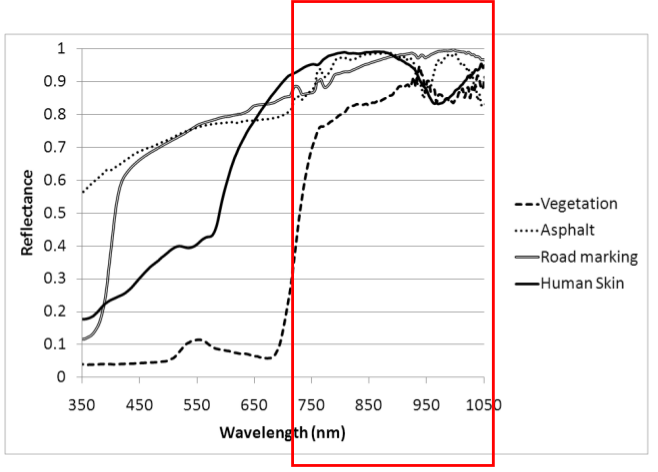
\includegraphics[width=0.7\textwidth, keepaspectratio=true]{chap6-Reflectance.png}
	\caption{Reflectance spectra of various substances.}
\end{figure}

\begin{figure}[h]
  \label{fig:chap6-humanskin}
  \centering
	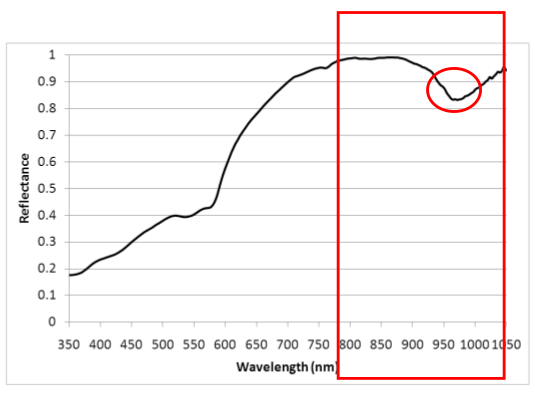
\includegraphics[width=0.7\textwidth, keepaspectratio=true]{chap6-humanskin.png}
	\caption{Reflectance spectra of human skin.}
\end{figure}

\begin{figure}[h]
  \label{fig:chap6-humanrace}
  \centering
	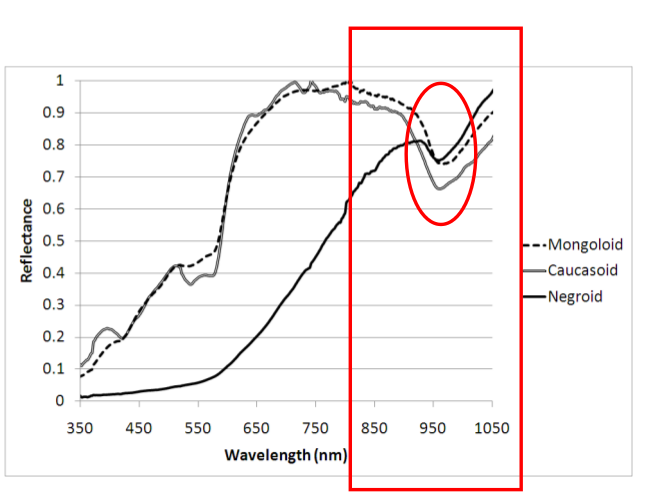
\includegraphics[width=0.7\textwidth, keepaspectratio=true]{chap6-humanrace.png}
	\caption{Spectra of various human skin.}
\end{figure}

\begin{figure}[h]
  \label{fig:chap6-mcam}
  \centering
	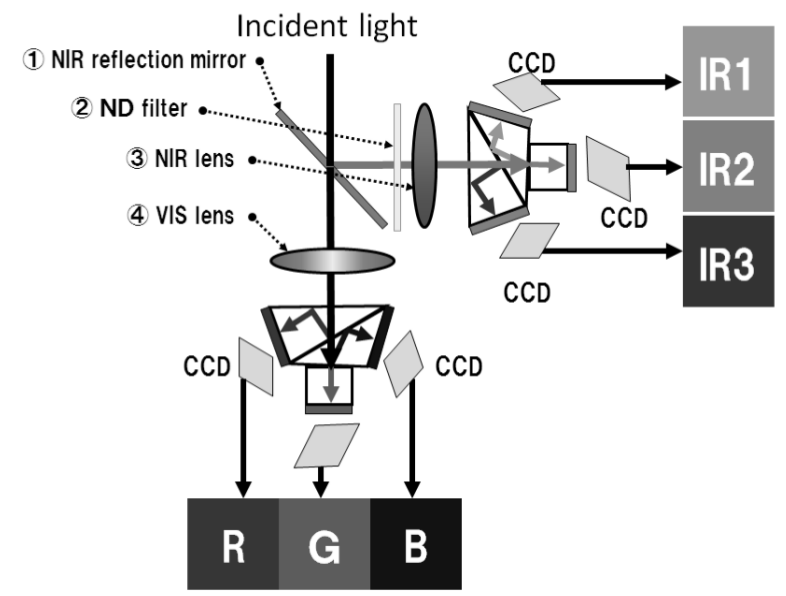
\includegraphics[width=0.7\textwidth, keepaspectratio=true]{chap6-mcam.png}
	\caption{Schematic diagram of the multi-camera module.}
\end{figure}
%----------------------------------------------------------------------------------------

\section{In Closing}

